%%%%%%%%%%%%%%%%%%%%%%%%%%%%%%%%%%%%%%%
% Wenneker Resume/CV
% LaTeX Template

% Original author:
% Frits Wenneker (http://www.howtotex.com) with extensive modifications by 
% Vel (vel@LaTeXTemplates.com)
%
% License:
% CC BY-NC-SA 3.0 (http://creativecommons.org/licenses/by-nc-sa/3.0/
%
%%%%%%%%%%%%%%%%%%%%%%%%%%%%%%%%%%%%%%

%----------------------------------------------------------------------------------------
%	PACKAGES AND OTHER DOCUMENT CONFIGURATIONS
%----------------------------------------------------------------------------------------

\documentclass[a4paper,12pt]{memoir} % Font and paper size

%%%%%%%%%%%%%%%%%%%%%%%%%%%%%%%%%%%%%%%%%
% Wenneker Resume/CV
% Structure Specification File
% Version 1.1 (19/6/2016)
%
% This file has been downloaded from:
% http://www.LaTeXTemplates.com
%
% Original author:
% Frits Wenneker (http://www.howtotex.com) with extensive modifications by 
% Vel (vel@latextemplates.com)
%
% License:
% CC BY-NC-SA 3.0 (http://creativecommons.org/licenses/by-nc-sa/3.0/)
%
%%%%%%%%%%%%%%%%%%%%%%%%%%%%%%%%%%%%%%%%%

%----------------------------------------------------------------------------------------
%	PACKAGES AND OTHER DOCUMENT CONFIGURATIONS
%----------------------------------------------------------------------------------------
\usepackage{hyperref}
\usepackage{fancyvrb}
\usepackage{XCharter} % Use the Bitstream Charter font
\usepackage[utf8]{inputenc} % Required for inputting international characters
\usepackage[T1]{fontenc} % Output font encoding for international characters

\usepackage[top=1cm,left=1cm,right=1cm,bottom=1cm]{geometry} % Modify margins

\usepackage{graphicx} % Required for figures

\usepackage{flowfram} % Required for the multi-column layout

\usepackage{url} % URLs

\usepackage[usenames,dvipsnames]{xcolor} % Required for custom colours

\usepackage{tikz} % Required for the horizontal rule

\usepackage{enumitem} % Required for modifying lists
\setlist{noitemsep,nolistsep} % Remove spacing within and around lists

\setlength{\columnsep}{\baselineskip} % Set the spacing between columns

% Define the left frame (sidebar)
\newflowframe{0.2\textwidth}{\textheight}{0pt}{0pt}[left]
\newlength{\LeftMainSep}
\setlength{\LeftMainSep}{0.2\textwidth}
\addtolength{\LeftMainSep}{1\columnsep}
 
% Small static frame for the vertical line
\newstaticframe{1.5pt}{\textheight}{\LeftMainSep}{0pt}
 
% Content of the static frame with the vertical line
\begin{staticcontents}{1}
\hfill
\tikz{\draw[loosely dotted,color=RoyalBlue,line width=1.5pt,yshift=0](0,0) -- (0,\textheight);}
\hfill\mbox{}
\end{staticcontents}
 
% Define the right frame (main body)
\addtolength{\LeftMainSep}{1.5pt}
\addtolength{\LeftMainSep}{1\columnsep}
\newflowframe{0.7\textwidth}{\textheight}{\LeftMainSep}{0pt}[main01]

\pagestyle{empty} % Disable all page numbering

\setlength{\parindent}{0pt} % Stop paragraph indentation

%----------------------------------------------------------------------------------------
%	NEW COMMANDS
%----------------------------------------------------------------------------------------

\newcommand{\userinformation}[1]{\renewcommand{\userinformation}{#1}} % Define a new command for the CV user's information that goes into the left column

\newcommand{\cvheading}[1]{{\Huge\bfseries\color{RoyalBlue} #1} \par\vspace{.6\baselineskip}} % New command for the CV heading
\newcommand{\cvsubheading}[1]{{\Large\bfseries #1} \bigbreak} % New command for the CV subheading

\newcommand{\Sep}{\vspace{1em}} % New command for the spacing between headings
\newcommand{\SmallSep}{\vspace{0.5em}} % New command for the spacing within headings

\newcommand{\aboutme}[2]{ % New command for the about me section
\textbf{\color{RoyalBlue} #1}~~#2\par\Sep
}
	
\newcommand{\CVSection}[1]{ % New command for the headings within sections
{\Large\textbf{#1}}\par
\SmallSep % Used for spacing
}

\newcommand{\CVItem}[2]{ % New command for the item descriptions
\textbf{\color{RoyalBlue} #1}\par
#2
\SmallSep % Used for spacing
}

\newcommand{\bluebullet}{\textcolor{RoyalBlue}{$\circ$}~~} % New command for the blue bullets
 % Include the file specifying document layout and packages

%----------------------------------------------------------------------------------------
%	NAME AND CONTACT INFORMATION 
%----------------------------------------------------------------------------------------

\userinformation{ % Set the content that goes into the sidebar of each page
\begin{flushright}

% Comment out this figure block if you don't want a photo
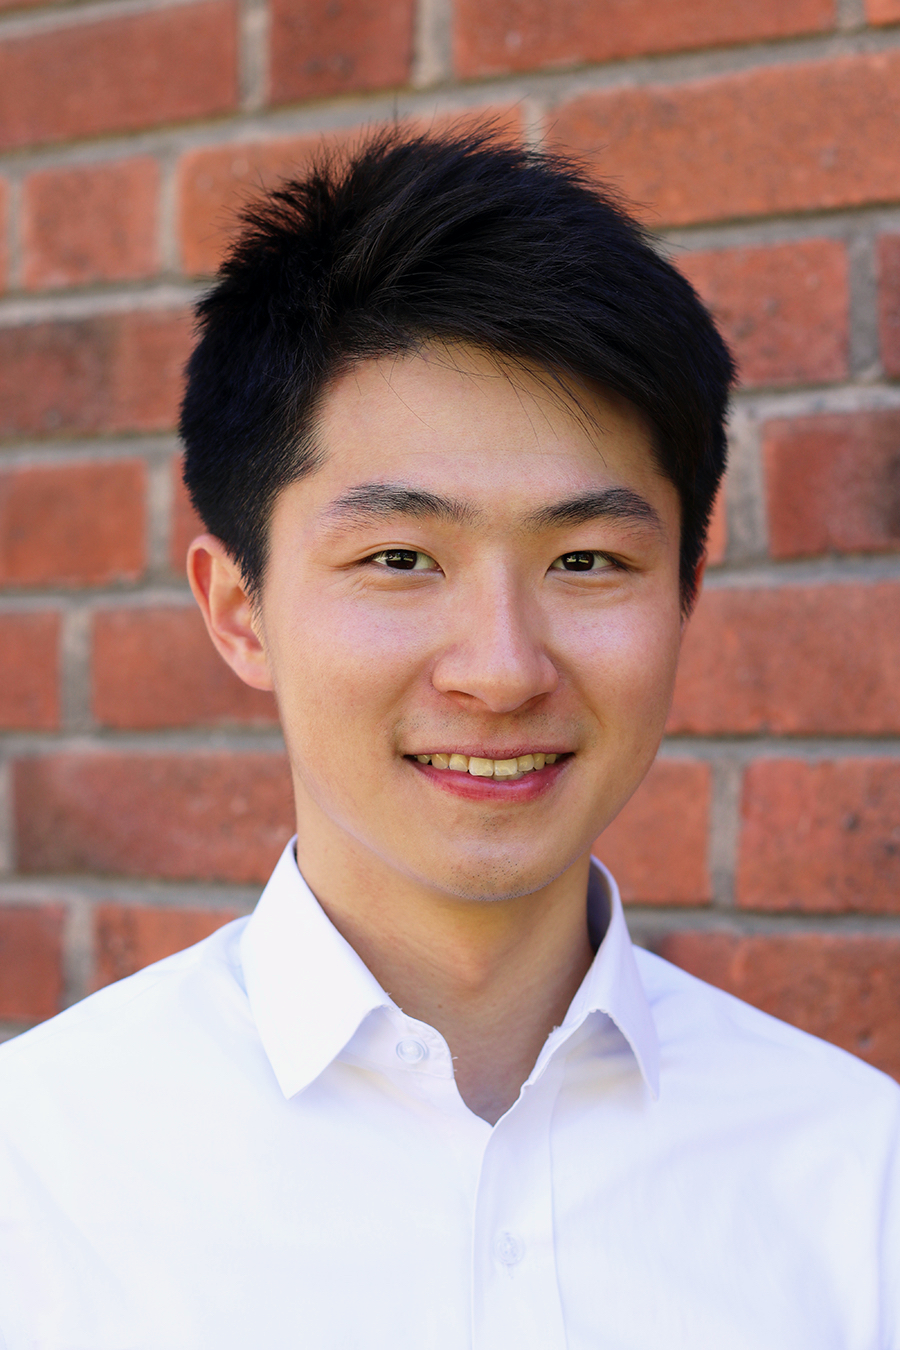
\includegraphics[width=1\columnwidth]{Enoch_Chen}\\[\baselineskip] % Your photo

\CVItem{Personal info} \\
\textbf{Enoch Yi-Tung Chen} \\ % Your name 
\href{https://linkedin.com/in/enoch-yi-tung-chen-299021157}{LinkedIn}
\href{https://enochytchen.com}{enochytchen.com} \\ % Your URL
\href{mailto:enoch.yitung.chen@ki.se}{enoch.yitung.chen@ki.se}\\
\href{tel:+46738774134}{+46 738774134} \\ % Your phone number

\vspace{1em}

\CVItem{Language} \\
Mandarin Chinese \\
English \\
Taiwanese  \\
Swedish (beginner)

\vspace{1em}

\CVItem{Software}\\
\Verb+Stata+ \\
\Verb+R+ \\
\LaTeX \\
\Verb+MS Office+ \\
\Verb+Git Hub+\\

\vfill % Whitespace under this block to push it up under the photo
\end{flushright}

}

%----------------------------------------------------------------------------------------

\begin{document}

\userinformation

\framebreak % End of the first column

%----------------------------------------------------------------------------------------
%	HEADING
%----------------------------------------------------------------------------------------

\cvheading{Enoch Yi-Tung Chen} % Large heading - your nae

%----------------------------------------------------------------------------------------
%	ABOUT ME
%----------------------------------------------------------------------------------------
\CVSection{Research interests}
{My main research interests are developing and applying statistical approaches for epidemiological studies in both register-based and trial-based settings, particularly in survival analysis and cost-effectiveness studies in health technology assessment.}

\vspace{1em}
%----------------------------------------------------------------------------------------
%	EDUCATION
%----------------------------------------------------------------------------------------

\CVSection{Education}

%------------------------------------------------

\CVItem{Karolinska Institutet \hspace*{\fill} 2018 - 2020}{MSc in Public Health Sciences, Epidemiology \\ Thesis: {\color{MidnightBlue}{\href{https://enochytchen.com/files/Enoch_MSc_thesis.pdf}{Extrapolating cancer patient survival: a comparison of the flexible parametric model and the rolling-over algorithm}}}}

%------------------------------------------------

\CVItem{National Taiwan University \hspace*{\fill} 2014 - 2018}{BSc in Public Health (Honour Graduate)}

\vspace{1em}
%----------------------------------------------------------------------------------------
%	EXPERIENCE
%----------------------------------------------------------------------------------------

\CVSection{Work \& Research}

%------------------------------------------------

\CVItem{Research Assistant \hspace*{\fill}Jun 2020 - present \\ 
							Department of Medical Epidemiology and Biostatistics (MEB) \\ Karolinska Institutet, Sweden}{
Achievements:
\begin{itemize}
	\item Completed {\color{MidnightBlue}{\href{https://enochytchen.com/tutorials/}{tutorials}}} on \href{https://enochytchen.com/tutorials/extrapolation/}{survival extrapolation}, \href{https://enochytchen.com/tutorials/relsurv/}{estimating relative survival}, \href{https://enochytchen.com/tutorials/ratetable/}{making ratetable using R}
	\item Teaching Assistant of Biostatistics workshops for med students
	\item Teaching {\color{MidnightBlue}{\href{https://enochytchen.com/courses/biostatbasics/}{\Verb+Stata+ lab session}}} in Applied Epidemiology course 
	\item Organised the Biostatistics Student Seminar at MEB
	\item Offered statistical assistance in  clinical epidemiological studies
	\item Writing a \Verb+Stata+ package called \Verb+translate hmd+ for creating population mortality files.
		\end{itemize}
\end{itemize}
}
\Sep
%------------------------------------------------
\CVItem{Project Intern \hspace*{\fill} Sep 2019 - Mar 2020 \\
		\href{https://synergusrwe.com}{Synergus Read-World Evidence}, Sweden}{Transferability studies in health technology assessment,
focusing on stroke healthcare delivery in Sweden.}

%------------------------------------------------
\Sep
\CVItem{Research Intern \hspace*{\fill}Jul - Aug 2019 \\
		Institute of Public Health, National Cheng Kung University, Taiwan}{Learned extrapolating cancer patients' survival, cost and quality of life using Taiwan's National Healthcare data}

%------------------------------------------------
\Sep
\CVItem{Fieldwork Intern \hspace*{\fill}Jul 2017 - Aug 2018\\
	    \href{https://lukeinternational.no}{Luke International Norway, Malawi}}{Sero-epidemiological study of dengue
prevalence in Northern Malawi}

%------------------------------------------------
\Sep
\CVItem{Principal Investigator \hspace*{\fill}Jul 2017 - Jun 2018}{Correlational study of class suspension and school enterovirus epidemic in Taiwan, 2010-2015 (honoured with College Student Research Creativity Award)}

\vspace{1em}

%----------------------------------------------------------------------------------------

\CVSection{Scholarships}
\CVItem{Karolinska Institutet Foundation \hspace*{\fill} 2019}

\CVItem{Alumni Association of National Taiwan University \hspace*{\fill} 2017}

\CVItem{Kung Pei Chen Preventive Medicine Foundation  \hspace*{\fill} 2016}

\end{document}
